\chapter{Conclusions}
\label{cha:conclussions}

En aquest cap\'{i}tol es descriu la evolució temporal, la gestió del projecte, la estimació econòmica i les possibles millores.


\section{Metodologia àgil}
Per la realització del projecte s'han emprat una metodologia \textit{agile}. Concretament aprofitant tècniques i artefactes de l'SCRUM.\cite{agile}\\

Els principis bàsics de la metodologia àgil són\cite{agilemanifesto}:
\begin{itemize}
\item Els individus i les seves interaccions per sobre dels processos i les eines.
\item El programari que funciona per sobre de la documentació exhaustiva.
\item La col·laboració amb el client per sobre de la negociació de contractes.
\item La resposta davant del canvi per sobre de seguir un pla tancat.
\end{itemize}

Per la realització d'aquest projecte s'han realitzat iteracions quinzenals amb el \textit{product owner}}.\cite{productowner} En cada iteració s'han anat canviant requisits, analitzant tecnologies, definint noves especificacions, definint nous requisits i fent petites \textit{demos} dels avanços implementats en cada iteració.\\

\subsection{Backlog}
En el cas d'aquest projecte s'ha usat l'artefacte principal ''Backlog'' mitjançant histories de usuaris. Les historia de usuari son una una representació d'un requisit del \textit{software} escrit en una o dos frases. En aquest cas:\\

\centerline{Com \textbf{rol} vull fer \textbf{alguna cosa} per \textbf{obtenir benefici}}
~\\
Ens hem basat en les histories d'usuaris amb el següent \textit{backlog} puntuant segons la serie de Fibonnaci.\cite{backlogfibonnacci}. Eludim els requeriments ja que es poden consultar al capitol \ref{cha:specification}.

\begin{center}
\begin{longtable}{ | p{3cm} | p{5cm} | p{5cm} | p{1cm} | }
\hline
\multicolumn{1}{|c|}{\textbf{Com}} & \multicolumn{1}{|c|}{\textbf{vull}} & \multicolumn{1}{|c|}{\textbf{per}} &\multicolumn{1}{|c|}{\textbf{Punts}} \\ \hline
Usuari anònim &	registrar-me &	usar la aplicació &	3 \\ \hline
Usuari registrat &	recuperar el password & entrar en cas que m'ho oblidi de la contrasenya & 3 \\ \hline
Usuari administrador &	vull afegir variables & indicar en les matrius quina variable de Ichnaea representa & 1 \\ \hline
Usuari registrat &	crear una matriu important un csv o excel & configurar-la i crear entrenaments & 8 \\ \hline
Usuari registrat &	crear un entrenament a partir d'una matriu & crear prediccions & 5 \\ \hline
Propietari d'una matriu & configurar una matriu & executar un entrenament & 21 \\ \hline
Propietari d'una matriu	& esborrar una matriu & eliminar dades, entrenaments i prediccions & 3 \\ \hline
Usuari registrat &	crear una predicció important un csv o excel & crear un conjunt de dades per predir i executar-es a Ichnaea & 8 \\ \hline
Propietari d'entrenament & 	esborrar una predicció & eliminar dades i prediccions & 2 \\ \hline
Usuari registrat & veure els resultat d'una predicció & consultar dades i crear una predicció & 1 \\ \hline
Usuari registrat & vull veure les matrius del sistema creades publiques & crear entrenaments a partir d'elles & 2  \\ \hline
Usuari registrat & vull veure els entrenaments finalitzats correctament	 & crear prediccions a partir d'elles & 2  \\ \hline
Usuari registrat & vull afegir conjunts de fitxers a un variable & indicar en les matrius quina conjunt de fitxers enviar a Ichnaea & 3  \\ \hline
Usuari registrat & vull esborrar fitxers d'un conjunt de fitxers & corregir dades en cas d'errors & 2 \\ \hline
Usuari administrador & vull testejar el sistema de cues & assegurar el correcte funcionament amb el sistema de cues en cas de detectar errors d'accesibilitat & 1 \\ \hline
Sistema de cues & vull indicar al sistema web que he acabat un entrenament & actulitzar les dades d'un entrenament i guardar els resultats al disc & 5 \\ \hline
Usuari registrat & enviar un predicció a la cua d'execucions de prediccions & predir origens de mostres & 5  \\ \hline
Usuari registrat & veure els resultats d'una predicció & consultar dades predites & 3  \\ \hline
Usuari registrat & veure un entrenament & consultar les dades entrenades i crear un predicció & 2  \\ \hline
Propietari d'un entrenament & vull enviar un entrenament a execució & poder crear prediccions & 5  \\ \hline
Sistema de cues & indicar al sistema web que tinc un resultat & poder consultar prediccions & 3  \\ \hline
Propietari d'una predicció & configurar les dades d'una matriu	& enviar les dades a Ichnaea per predir & 21  \\ \hline
Propietari d'una matriu & validar la matriu	 & comprovar la validessa de les dades & 5  \\ \hline
\caption{Taula de \textit{backlog} ponderada amb la serie de Fibonnaci}
\end{longtable}
\end{center}

\section{Planificació}
A la figura \ref{fig:gant} es descriu la planificació àgil per setmanes i per ítems.
\begin{sidewaysfigure}[ht]
    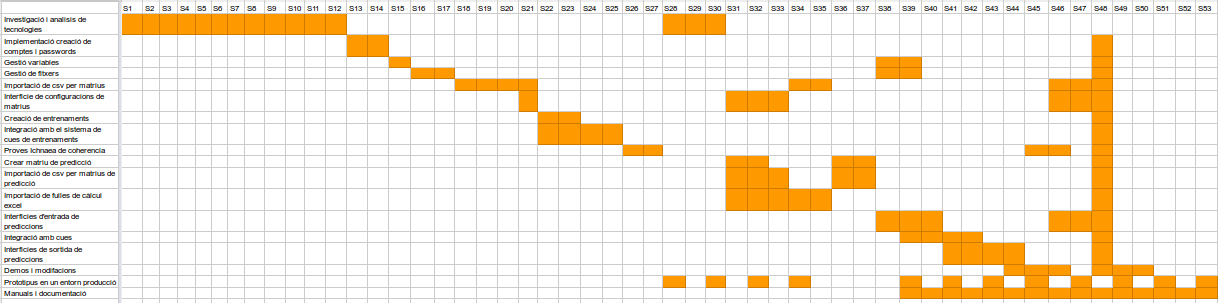
\includegraphics[scale=0.5]{img/conclussions/gantz.png}
    \caption{Diagrama de Gant.}
    \label{fig:gant}
\end{sidewaysfigure}

Al contrari de les metodologies en cascada, a on no es passa al següent ítem fins que s'acabi, es pot veure com es modifica ítems anteriors segons els canvis en cada iteració \textit{agile}.

\section{Estimaci\'{o} econ\'{o}mica}
La estimació del cost es calcula a partir dels següents paràmetres:
\begin{itemize}
\item Cada setmana de desenvolupament del projecte son 15 hores
\item Calcul a partir del cost. Es contempla com a cost intern seguint el cost dels rols involucrats en cada àrea.
\item Calcul de venta com a servei. Es contempla el cas de venta de projecte com empresa segons els preus de mercats d'una consultoria \textit{StartUp} de desenvolupament a mida.
\item Es un projecte àgil. Tots els integrants treballen en totes les tareas.
\item Son iteracions r\'{a}pides de dues setmanes.
\end{itemize}

\begin{sidewaystable}
\begin{tabular}{|p{3cm}|p{2cm}|p{1cm}|p{3cm}|p{1cm}|p{2cm}|p{2cm}|p{2cm}|p{2cm}|}
\hline
Tarea & Setmanes & Hores & Rols & Cost \euro/h & Cost total & Servei \euro/h & Servei total & Rendiment \\ \hline
Especificacions i tomes de requeriments & N/A: 3 hores per iteració & 91.5 h & Cap de projecte & 18 \euro/h & 1647\euro & 45 \euro/h & 4117.5\euro & \\ \hline
Anàlisis de tecnologia & 15 setmanes & 225 h & Analista & 15 \euro/h & 3375\euro & 30\euro & 6750\euro & \\ \hline
Implementació Aplicació & 32 setmanes & 480 h & Desenvolupador & 12 \euro/h & 5760 & 30\euro/h & 14440\euro & \\ \hline
Documentació i Qualitat & 14 setmanes & 210 h & Becari & 8 \euro/h & 1680\euro & & & \\ \hline 
\hline
Total & 61 setmanes & 1006.5 h & & & 12462\euro & & 25267.5\euro & 12805.5\euro \\ \hline
\end{tabular}
\end{sidewaystable}

\section{Millores en futures versions}
A continuació es dona una breu descripció de possibles treballs futurs d'aquest projecte.
\begin{itemize}
\item Refactoritzaci\'{o} del codi
\item Personalitzaci\'{o} dels perfils d'usuari: formats de dades, dates, idiomes en el cas de internalitzaci\'{o}
\item Ampliaci\'{o} de les API Restful
\item Depuraci\'{o} en els exploradors m\'{e}s habituals. La aplicaci\'{o} est\'{a} depurada per Mozilla Firefox i Google Chrome. Per\'{o} no ha sigut per Internet Explorer o Safari.
\item Depuraci\'{o} en entorn distribuït del sistema de cues. Encara que la aplicaci\'{o} ha sigut desenvolupada per ser distribuïda i separada del sistema de cues, no ha sigut possible provar-la en un entorn m\'{e}s complexe i distribuït.
\item Sistema de notificacions. Un sistema m\'{e}s el.laborat de notificacions. Per exemple, notificacions quan un ''training'' ha acabat o enviar
\item Sistema de projectes. La aplicaci\'{o} no ha sigut contemplada per ser m\'{e}s col.laborat-iva. Hauria de ser m\'{e}s concurrent contra alguns recursos, per exemple diversos editors d'una matriu al mateix temps.
\item Sistema de invitacions. Un sistema per invitar col.laboradors tant siguin de la plataforma com si no.
\item Implementar tests autom\'{a}tics.
\end{itemize}

\section{Conclusions finals}
La realització d'aquest projecte esta motivada per la evolució d'Ichnaea com a sistema complexe. Durant la realització d'aquest projecte s'han pogut observar les 
